%------------------------------------------------------------------------
%Editar Diplomado
\hypertarget{cv:terminarCU}{\section{Terminar Caso de uso}} \label{sec:terminarCU}

	Esta funcionalidad le permitirá mandar a revisión un caso de uso que se ha completado para su validación.
		\subsection{Procedimiento}

			%Pasos de procedimiento
			\begin{enumerate}
			
			\item Oprima el botón \IUTerminar{} de algún registro existente de la pantalla \ref{fig:GestionarCU} ''Gestionar Casos de Uso''.
	
			\item Se mostrará el mensaje \ref{fig:confirmaTerminaCU} sobre la pantalla \ref{fig:GestionarCU} ''Gestionar Casos de Uso''.
			
			%Pantalla
			\begin{figure}[htbp!]
				\begin{center}
					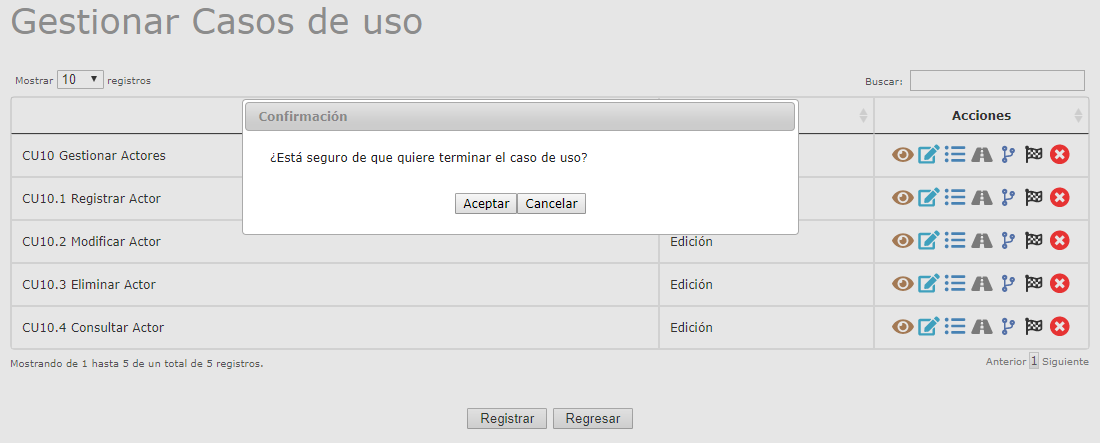
\includegraphics[scale=0.6]{roles/lider/casosUso/pantallas/IU12-5MSG10}
					\caption{MSG de Confirmación}
					\label{fig:confirmaTerminaCU}
				\end{center}
			\end{figure}
				
				\item Oprima el botón \IUAceptar.
				
				\item Se mostrará el mensaje \ref{fig:CUTerminado} en la pantalla \ref{fig:GestionarCU} ''Gestionar Casos de Uso''.
				
				\begin{figure}[htbp!]
					\begin{center}
						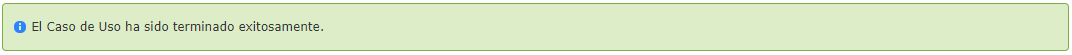
\includegraphics[scale=0.6]{roles/lider/casosUso/pantallas/IU12-5MSG1}
						\caption{MSG: Caso de Uso Terminado}
						\label{fig:CUTerminado}
					\end{center}
				\end{figure}
			
			\end{enumerate}